\usetikzlibrary{arrows,automata,positioning}
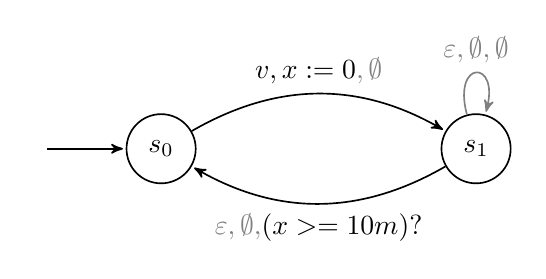
\begin{tikzpicture}[->,>=stealth',shorten >=1pt,auto,node distance=4cm, semithick]
	\node(start) {};
	\node[state] (S0) [right=0cm and 1cm of start]{$s_0$};
	\node[state](S1) [right of=S0] {$s_1$};

	\path (start) edge node {} (S0);
	\path (S0) edge [bend left] node {$v, x := 0 \textcolor{gray}{, \emptyset}$} (S1);
	\path (S1) edge [bend left] node {$\textcolor{gray}{\varepsilon, \emptyset, }(x >= 10m)?$} (S0);
	\path (S1) edge [color=gray,loop above] node {$\varepsilon, \emptyset, \emptyset$} (S1);
\end{tikzpicture}
